%//==============================--@--==============================//%
%\vspace{-1em}
\subsection{P2 | Validação do programa.}
\label{subsec:P2}

%//==============================--A--==============================//%
%\vspace{-0.5em}
\subsubsection{i) Coerência entre a sequência dos estados ao longo das várias jogadas e a sequência de eventos que a determinam.}
\label{subsubsec:P2i}

A transição entre estados depende de um acontecimento definido probabilisticamente (o lançamento da moeda). Complementamos a \hyperref[subsec:intro]{matriz de transição} com a \hyperref[tab:state-transitions]{Tab. 1.:}

\begin{wraptable}[11]{l}{5.5cm}
  \centering
  \label{tab:state-transitions}
  \caption{Transição de estados.}
  \begin{tabular}{ccc}
    \toprule
          & \multicolumn{2}{c}{$\pmb{x_{j+1}}$} \\
    $\pmb{x_j}$ & Cara  & Coroa \\ \midrule
    $x_1$ & $x_2$ & $x_3$ \\
    $x_2$ & $x_3$ & $x_4$ \\
    $x_3$ & $x_4$ & $x_5$ \\
    $x_4$ & $x_5$ & $x_6$ \\
    $x_5$ & $x_6$ & $x_3$ \\
    $x_6$ & $x_3$ & $x_7$ \\
    $x_7$ & $x_1$ & $x_2$ \\ \bottomrule
  \end{tabular}
\end{wraptable}

\noindent $\rightarrow$ \textbf{\textit{Observações}}

\begin{itemize}
    \item[$\blacktriangle$] Afluem quatro estados para $x_3$: 
    \vspace{-0.35em}
    $$ \pi_3 = \dfrac{1}{2}\left(\pi_1 + \pi_2 + \pi_5 + \pi_6\right) $$

    \vspace{-1em}\item[$\blacktriangle$] É apenas possível transitar para os estados $x_2$, $x_4$, $x_5$ e $x_6$ através dos dois estados anteriores:
    \vspace{-1.15em}
    \begin{gather*}
        \pi_2 = \frac{1}{2}(\pi_1 + \pi_7)\qquad\pi_4 = \frac{1}{2}(\pi_2 + \pi_3) \\
        \pi_5 = \frac{1}{2}(\pi_3 + \pi_4)\qquad\pi_6 = \frac{1}{2}(\pi_4 + \pi_5)
    \end{gather*}

    \vspace{-1em}\item[$\blacktriangle$] Transita-se para $x_1$ de $x_7$ e para $x_7$ de $x_6$:
    \vspace{-0.35em}
    $$ \pi_1 = \frac{1}{2}\pi_7 = \frac{1}{2}\left(\frac{1}{2}\pi_6\right) $$
\end{itemize}

A validação dos resultados \hyperref[subsubsec:P1b]{advindos da simulação} e \hyperref[subsec:intro]{deduzidos teoricamente} é naturalmente observada com as relações expostas acima.
%//==============================--A--==============================//%
%\vspace{-0.5em}
\subsubsection{ii) Convergência da distribuição das probabilidades dos diferentes estados com o aumento do número de \textit{runs} de Monte Carlo.}
\label{subsubsec:P2ii}

A convergência da distribuição das probabilidades dos diferentes estados é estudada através do \textit{root mean square error} (\textit{RMSE}) acumulado ao longo de $N$ \textit{runs} de Monte Carlo (NMC)\footnotemark[3]:

%//==============================--A--==============================//%
\footnotetext[3]{Para \textit{runs} de 200 jogadas totais.}
%//==============================--A--==============================//%

\begin{figure}[H] 
    \begin{subfigure}[b]{0.5\linewidth}
        \centering
        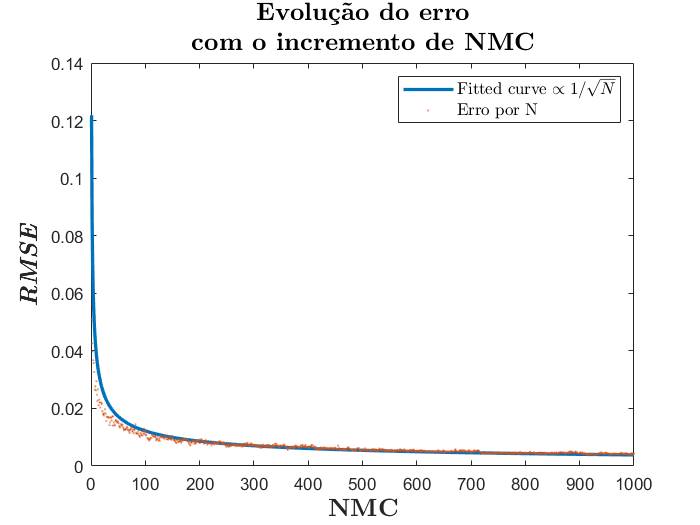
\includegraphics[width=1\linewidth]{img/P2/P2ii-discard.png}
        \caption{Evolução do erro ao longo de N \textit{runs} de Monte Carlo} 
        \label{fig:P2ii} 
        \vspace{1ex}
    \end{subfigure}%% 
    \begin{subfigure}[b]{0.5\linewidth}
        \centering
        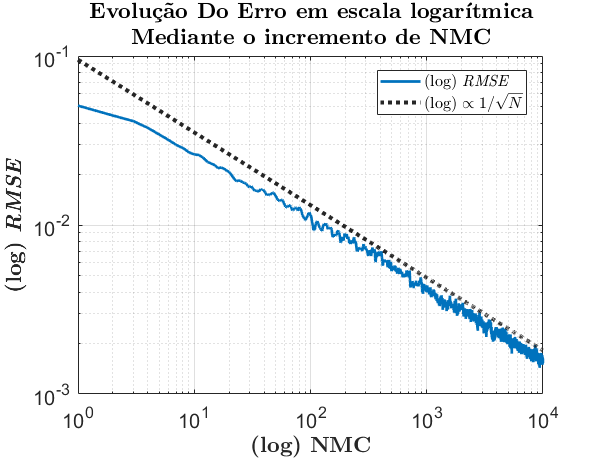
\includegraphics[width=1\linewidth]{img/P2/P2iilog.png} 
        \caption{Evolução do erro em escala logarítmica.} 
        \label{fig:P2ii-log} 
        \vspace{1ex}
    \end{subfigure} 
    \caption{Ilustração da \textit{convergence rate} da Cadeia de Markov.}
\end{figure}

\noindent\textbf{\textit{$\rightarrow$ Observações}}

\begin{itemize}
    \item[$\blacktriangle$] A \textit{fitted curve} demonstra que o decaimento do erro tem um \textit{rate} $\propto\, 1/\sqrt{N}$ (onde $N$ são as \textit{runs} de Monte Carlo) $\rightarrow$ O \textit{convergence rate} dos diferentes estados é da ordem de $\mathcal{O}(1/\sqrt{N})$, realidade independente da dimensão da cadeia:
\end{itemize}
\begin{quote}
    ``Monte Carlo's convergence rate, $\mathcal{O}(1/\sqrt{N})$, is independent of dimension.''\cite{caflisch_2008}
\end{quote}

\begin{itemize}
    \item[$\blacktriangle$] A visualização dos eixos no espaço logarítmico (vide \hyperref[fig:P2ii-log]{Fig. 5 b)}) sugere que para valores elevados de $N$ a aproximação à reta $\propto\: 1/\sqrt{N}$ torna-se cada vez mais refinada.
\end{itemize}

Estudou-se ainda a evolução do erro para \textit{seeds} diferentes, de forma a variar o gerador de números aleatórios:

\begin{figure}[H]
    \centering
    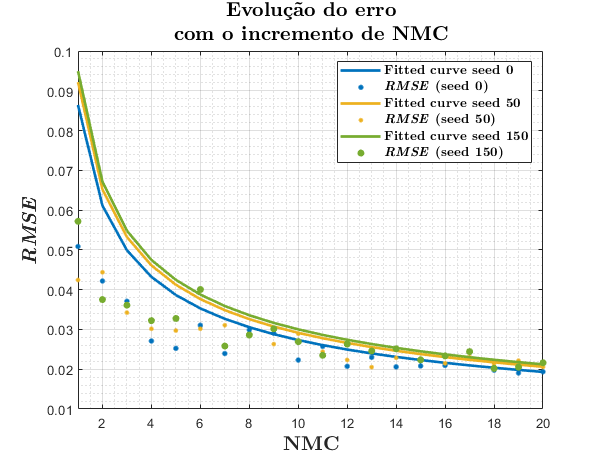
\includegraphics[width = 0.6\linewidth]{img/P2/P2iiseed.png}
    \caption{Convergence rate para \textit{seeds} diferentes.}
    \label{fig:seed}
\end{figure}

\noindent\textbf{\textit{$\rightarrow$ Observações}}

\begin{itemize}
    \item[$\blacktriangle$] A variação do gerador de números aleatórios não afeta a evolução do erro mediante o número de NMC's: as \textit{fitted curves} demonstram sempre que o decaimento do erro tem um \textit{rate} $\propto\: 1/\sqrt{N}$. A não sobreposição aparente das \textit{fitted curves} advém da sequência de números aleatórios distintos, consequentemente, valores de \textit{RMSE} distintos.
\end{itemize}

\vspace{-1.5em}
\subsubsection{iii) Valor adequado da variável Ndiscard.}
\label{subsubsec:P2iii}

\textit{Ndiscard}, normalmente conhecido pelo termo \textit{burn-in}/\textit{warm-up}, destina-se a dar tempo suficiente à Cadeia de Markov para atingir o seu \textit{steady-state}/\textit{equilibrium distribution}, livre do \textit{bias} inicial imposto pelo estado de partida:

\begin{quote}
 \textit{``The idea is that a "bad" starting point may over-sample regions that are actually very low probability under the equilibrium distribution before it settles into the equilibrium distribution. If you throw those points away, then the points which should be unlikely will be suitably rare.''}\cite{amelio}
\end{quote}

Procuramos um número de iterações grande o suficiente para garantir uma cadeia bem misturada, o que se traduz num \textit{RMSE} (\textit{root mean square error}) mínimo:
\newpage
$\rightarrow$ Ao realizar $N$ simulações de Monte Carlo\footnotemark[4], cada uma com \textit{burn-in} incrementalmente diferente, \textbf{pretendemos depreender uma gama de valores de \textit{Ndiscard} para o qual o erro é mínimo e estável.}

\begin{figure}[H]
    \centering
    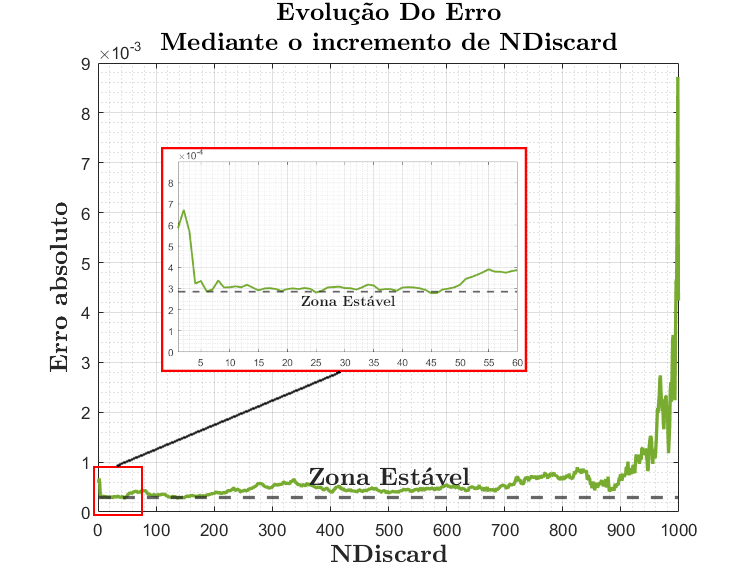
\includegraphics[width = 0.6\linewidth]{img/P2/P2iii.png}
    \caption{Erro absoluto mediante o incremento de \textit{Ndiscard} para simulações de 1000000 \textit{runs} e 1000 jogadas totais. (\textbf{\underline{Nota}:} foi omitido o valor do erro absoluto para \textit{Ndiscard }$= 1000$ de forma a uma melhor visualização do comportamento da evolução do erro. Tal será esperado nas subsequentes figuras.)}
    \label{fig:P2iii}
\end{figure}

\noindent\textbf{\textit{$\rightarrow$ Observações}}

\begin{itemize}
    \item[$\blacktriangle$] Para \textit{Ndiscard} < 5 é identificada uma forte flutuação de erros $\rightarrow$ o regime transitório influência os valores de frequência relativa estimados.
    \item[$\blacktriangle$] Para \textit{Ndiscard} $\in\ ]5, 60]$ o erro calculado atinge uma estabilidade mínima correspondente à gama de valores já supramencionada.
    \item[$\blacktriangle$] Para \textit{Ndiscard} > 60 A regressão do erro torna-se progressivamente maior e mais instável, com um pico na gama $[900,1000[$. Este comportamento é trivialmente explicado pela natureza da Cadeia de Markov: Ao descartar um número de jogadas próximo do seu valor total (1000), a ponderação da probabilidade tem por base um número de amostras reduzido. Reconhecendo que a \textit{equilibrium distribuition} da Cadeia de Markov só é atingida para um elevado valor de transições\footnotemark[5] a estimativa da probabilidade apresenta maior incidência de erro.
\end{itemize}

Por outro lado, a literatura indica que:

\begin{quote}
   \textit{``The amount that should be thrown away is usually less than 1\% of a run whenever a run is long enough to give enough precision. So routinely throwing away the initial 1\% or 2\% of runs will usually suffice.''}\cite{Geyer1992}
\end{quote}

\underline{Logo é admitido um valor ótimo de \textit{Ndiscard} de 20.}
\\\\
\textbf{\textit{$\rightarrow$ Nota:}}
\\
O método de Monte Carlo supõe um elevado número de \textit{runs}\footnotemark[6] para um valor de \textit{Njogadas} satisfatório, podemos ainda admitir o estudo do comportamento do número de erros para duas instâncias diferentes, \textit{Many short runs} e \textit{Few long runs}:

\begin{figure}[H] 
    \begin{subfigure}[b]{0.5\linewidth}
        \centering
        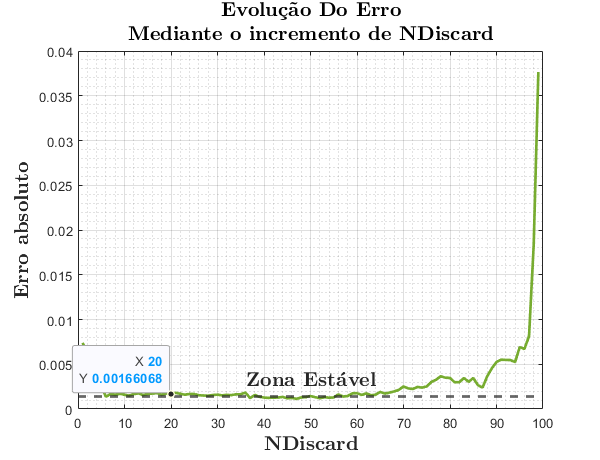
\includegraphics[width=1\linewidth]{img/P2/P2iiishort.png}
        \caption{\textit{Many short runs}:\\ \textit{NMC} = 100000, \textit{Njogadas total} = 100} 
        \label{fig:short} 
        %\vspace{1ex}
    \end{subfigure}%% 
    \begin{subfigure}[b]{0.5\linewidth}
        \centering
        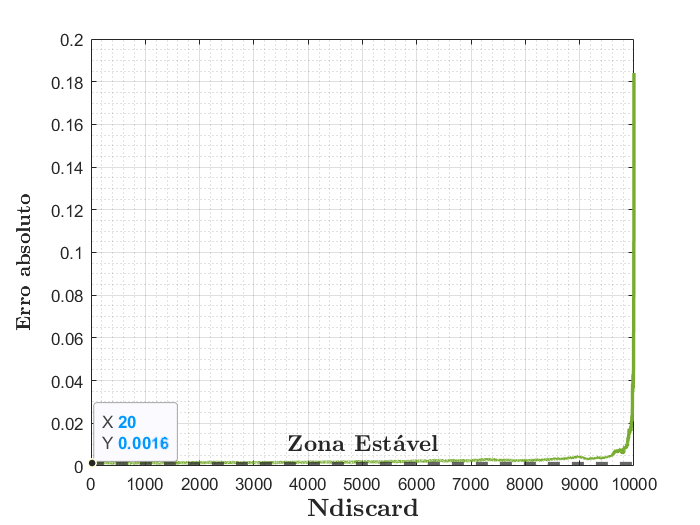
\includegraphics[width=1\linewidth]{img/P2/P2iiilong.png} 
        \caption{\textit{Few long runs}:\\ \textit{NMC} = 100, \textit{Njogadas total} = 100000} 
        \label{fig:Long} 
        %\vspace{1ex}
    \end{subfigure} 
    \caption{Comportamento do número de erros para as duas instâncias.}
    \label{fig:COMPARENdiscard}
\end{figure}

Embora o erro para um \textit{Ndiscard} de 20 seja satisfatório para as duas instâncias já acima referidas é importante compreender que o valor de \textit{burn-in} escolhido é totalmente inerente ao tipo de simulação realizada\footnotemark[7]. Para o P1 são admitidas simulações de 1000000 \textit{runs}, 1000 \textit{Njogadas total} e 20 \textit{Ndiscard} \textbf{(\textit{Many short runs}) já que a \textit{convergence rate} é de $\mathcal{O}(1/\sqrt{N})$ onde $\pmb{N}$ é o número de \textit{runs} de Monte Carlo.}

%//==============================--A--==============================//%
\footnotetext[4]{Entendemos por simulação uma simulação onde decorrem n \textit{runs} de Monte Carlo.}
\footnotetext[5]{Vide \hyperref[subsec:intro]{secção introdutória}.}
\footnotetext[6]{Procuramos simular a Cadeia de Markov NMC (\textit{N de Monte Carlo, número de runs}) vezes.}
\footnotetext[7]{Tipo de Cadeia de Markov, número de \textit{runs} e número de \textit{Njogadas total}.}
%//==============================--A--==============================//%
%\vspace{-0.5em}
\subsubsection{iv) Outros aspetos importantes.}
\label{subsubsec:P2iv}

\noindent\textbf{\textit{$\rightarrow$ Métodos de diagnóstico}}\\
Na literatura, a estimação do \textit{burn-in}/\textit{warm-up}, bem como, da região de convergência da Cadeia de Markov é efetuada mediante diversos padrões de diagnóstico, tais como: \textit{trace plot}, \textit{autocorrelation}... Infelizmente não abordados, devido à \textit{scope} do problema.

\vspace{1em}
\noindent\textbf{\textit{$\rightarrow$ Fórmulas de erro escolhidas}}
\begin{align*}
    \text{RMSE}&\delequal \; \sqrt{\frac{1}{\text{NMC}}\sum\limits_{n=1}^{\text{NMC}}\left\parallel\pmb{\hat{\pi}}_n - \pmb{\pi}_{\text{teo.}}\!\right\parallel} \\
    \text{Erro absoluto}&\delequal \; \sum\limits_{j=1}^{\text{Ncasas}} \left\vert \hat{\pi}_j - \pi_{\text{teo.},j} \right\vert
\end{align*}

O \textit{RMSE} foi escolhido para visualizar a \textit{convergence rate} da distribuição das probabilidades dos diferentes estados dado que pode ser visto como a distância (assemelhando-se à Euclidiana, mas \textit{rescaled}/\textit{normalized}) entre o vetor simulado e o \hyperref[subsec:intro]{vetor teórico esperado}.

O erro absoluto propiciou uma melhor visualização da região de transição prevista na evolução do erro mediante o incremento de \textit{Ndiscard}.
%//==============================--@--==============================//%